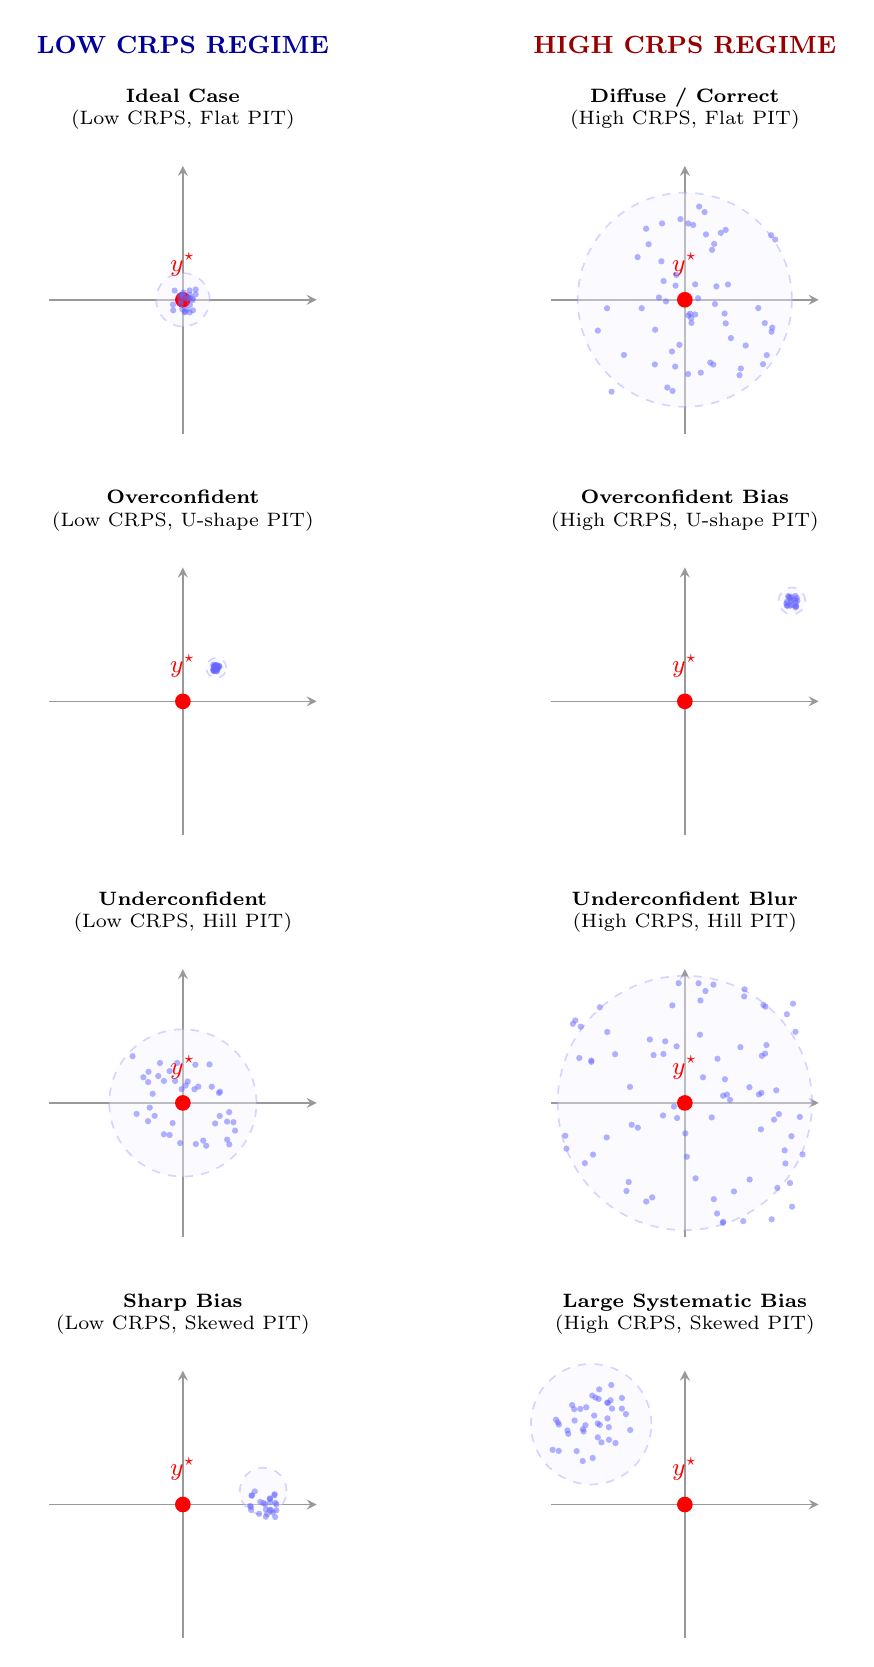
\begin{tikzpicture}[font=\sffamily, scale=0.85]

% --- Global Styles ---
\tikzset{
    axis/.style={->, >=stealth, line width=0.6pt, gray!80},
    % Enlarged Target Style as requested
    target/.style={circle, fill=red, inner sep=2pt, label={[red, font=\small, yshift=2pt]above:$\vect{y}^\star$}},
    candidate/.style={circle, fill=blue!60, opacity=0.5, inner sep=0.8pt},
    dispersion/.style={draw=blue!40, fill=blue!5, dashed, line width=0.6pt, opacity=0.4}
}

% ==============================================================================
% LEFT COLUMN: LOW CRPS (Sharp / Generally Accurate)
% ==============================================================================

% CASE 1: Ideal
\begin{scope}[shift={(0,0)}]
    \draw[axis] (-2,0) -- (2,0); \draw[axis] (0,-2) -- (0,2);
    \node[anchor=south, font=\scriptsize, align=center] at (0,2.4) {\textbf{Ideal Case} \\ (Low CRPS, Flat PIT)};
    \draw[dispersion] (0,0) circle (0.4);
    \node[target] at (0,0) {};
    \foreach \i in {1,...,25} \node[candidate] at (0.2*rand, 0.2*rand) {};
\end{scope}

% CASE 2: Overconfident
\begin{scope}[shift={(0,-6.0)}]
    \draw[axis] (-2,0) -- (2,0); \draw[axis] (0,-2) -- (0,2);
    \node[anchor=south, font=\scriptsize, align=center] at (0,2.4) {\textbf{Overconfident} \\ (Low CRPS, U-shape PIT)};
    \draw[dispersion] (0.5, 0.5) circle (0.15);
    \node[target] at (0,0) {};
    \foreach \i in {1,...,25} \node[candidate] at (0.5 + 0.05*rand, 0.5 + 0.05*rand) {};
\end{scope}

% CASE 3: Underconfident
\begin{scope}[shift={(0,-12.0)}]
    \draw[axis] (-2,0) -- (2,0); \draw[axis] (0,-2) -- (0,2);
    \node[anchor=south, font=\scriptsize, align=center] at (0,2.4) {\textbf{Underconfident} \\ (Low CRPS, Hill PIT)};
    \draw[dispersion] (0,0) circle (1.1);
    \node[target] at (0,0) {};
    \foreach \i in {1,...,40} \node[candidate] at (0.8*rand, 0.8*rand) {};
\end{scope}

% CASE 4: Sharp Bias
\begin{scope}[shift={(0,-18.0)}]
    \draw[axis] (-2,0) -- (2,0); \draw[axis] (0,-2) -- (0,2);
    \node[anchor=south, font=\scriptsize, align=center] at (0,2.4) {\textbf{Sharp Bias} \\ (Low CRPS, Skewed PIT)};
    \draw[dispersion] (1.2, 0.2) circle (0.35);
    \node[target] at (0,0) {};
    \foreach \i in {1,...,25} \node[candidate] at (1.2 + 0.2*rand, 0.2*rand) {};
\end{scope}

% ==============================================================================
% RIGHT COLUMN: HIGH CRPS (Diffuse / High Error)
% ==============================================================================

% CASE 5: Diffuse
\begin{scope}[shift={(7.5,0)}]
    \draw[axis] (-2,0) -- (2,0); \draw[axis] (0,-2) -- (0,2);
    \node[anchor=south, font=\scriptsize, align=center] at (0,2.4) {\textbf{Diffuse / Correct} \\ (High CRPS, Flat PIT)};
    \draw[dispersion] (0,0) circle (1.6);
    \node[target] at (0,0) {};
    \foreach \i in {1,...,60} \node[candidate] at (1.4*rand, 1.4*rand) {};
\end{scope}

% CASE 6: Overconfident Bias
\begin{scope}[shift={(7.5,-6.0)}]
    \draw[axis] (-2,0) -- (2,0); \draw[axis] (0,-2) -- (0,2);
    \node[anchor=south, font=\scriptsize, align=center] at (0,2.4) {\textbf{Overconfident Bias} \\ (High CRPS, U-shape PIT)};
    \draw[dispersion] (1.6, 1.5) circle (0.2);
    \node[target] at (0,0) {};
    \foreach \i in {1,...,20} \node[candidate] at (1.6+0.1*rand, 1.5+0.1*rand) {};
\end{scope}

% CASE 7: Underconfident Blur
\begin{scope}[shift={(7.5,-12.0)}]
    \draw[axis] (-2,0) -- (2,0); \draw[axis] (0,-2) -- (0,2);
    \node[anchor=south, font=\scriptsize, align=center] at (0,2.4) {\textbf{Underconfident Blur} \\ (High CRPS, Hill PIT)};
    \draw[dispersion] (0,0) circle (1.9);
    \node[target] at (0,0) {};
    \foreach \i in {1,...,80} \node[candidate] at (1.8*rand, 1.8*rand) {};
\end{scope}

% CASE 8: Systematic Failure
\begin{scope}[shift={(7.5,-18.0)}]
    \draw[axis] (-2,0) -- (2,0); \draw[axis] (0,-2) -- (0,2);
    \node[anchor=south, font=\scriptsize, align=center] at (0,2.4) {\textbf{Large Systematic Bias} \\ (High CRPS, Skewed PIT)};
    \draw[dispersion] (-1.4, 1.2) circle (0.9);
    \node[target] at (0,0) {};
    \foreach \i in {1,...,40} \node[candidate] at (-1.4+0.6*rand, 1.2+0.6*rand) {};
\end{scope}

% --- Main Column Headers ---
\node[font=\small\bfseries, blue!60!black] at (0, 3.8) {LOW CRPS REGIME};
\node[font=\small\bfseries, red!60!black] at (7.5, 3.8) {HIGH CRPS REGIME};

\end{tikzpicture}